\documentclass[11pt]{article}

% ---------- PACKAGES ----------
\usepackage[a4paper,margin=2.5cm]{geometry}
\usepackage{titlesec}
\usepackage{enumitem}
\usepackage{booktabs}
\usepackage{longtable}
\usepackage{array}
\usepackage{xcolor}
\usepackage{hyperref}
\usepackage{parskip}
\usepackage{fancyhdr}
\usepackage[backend=biber, style=ieee]{biblatex}
\addbibresource{references.bib}   % with .bib here
\usepackage{graphicx}

% ---------- COLORS ----------
\definecolor{tumblue}{RGB}{0,101,189}
\definecolor{openq}{RGB}{178,34,34}
\definecolor{vincenzoq}{RGB}{204,153,0}
\definecolor{todo}{RGB}{0,120,90}
\definecolor{review}{RGB}{128,0,128}

% ---------- HYPERLINK STYLE ----------
\hypersetup{
    colorlinks=true,
    linkcolor=tumblue,
    urlcolor=tumblue,
    citecolor=tumblue
}

% ---------- SECTION STYLE ----------
\titleformat{\section}{\Large\bfseries\color{tumblue}}{\thesection}{1em}{}
\titleformat{\subsection}{\large\bfseries\color{tumblue!80!black}}{\thesubsection}{1em}{}

% ---------- HEADER / FOOTER ----------
\pagestyle{fancy}
\fancyhf{}
\fancyhead[L]{Month 2 Delivery}
\fancyhead[R]{Ines Suarez Garcia}
\fancyfoot[C]{\thepage}
\renewcommand{\headrulewidth}{0.4pt}
\setlength{\headheight}{14pt}

% ---------- CUSTOM COMMANDS FOR TRACKING ----------
\newcommand{\openquestion}[1]{\textcolor{openq}{\textbf{Open question:}} #1}
\newcommand{\vincenzoq}[1]{\textcolor{vincenzoq}{\textbf{Open question to Vincenzo:}} #1}
\newcommand{\actionitem}[1]{\textcolor{todo}{\textbf{Action item:}} #1}
\newcommand{\status}[1]{\textit{\textcolor{gray}{Status: #1}}}
\newcommand{\review}[1]{\textcolor{review}{\textbf{Review this:}} #1}


\title{\textbf{Optimal Central-Node Placement in ISL-Connected \\ Distributed Satellite Systems} \\[0.3cm] \large Master Thesis: Month 2 Delivery}
\author{Ines Suarez Garcia \\ TUM Chair of Spacecraft Systems / NeuralAgent}
\date{Last updated: \today}

\begin{document}

\maketitle

\begin{center}
\textcolor{gray}{\textbf{Supervisors:} Vincenzo Messina (TUM), Indraditya Bhattacharyya (NeuralAgent), Harald Bayerlein (NeuralAgent)}
\end{center}

\vspace{0.5cm}

% =========================================================
\section{Progress Since Month 1}
% =========================================================

This report builds on the Month 1 Delivery, whose scope, research questions, dataset selection and baseline proposal remain valid and are not repeated here. During Month 2 the work has focused on the following points:
\begin{itemize}[leftmargin=1.2cm]
    \item \textbf{Sensor field of view.} The FOV of each sensing satellite has been implemented, so that observation opportunities are now driven by the sensor geometry rather than by the communication elevation mask (Section~\ref{sec:eo}).
    \item \textbf{Ground segment.} Five ground stations have been implemented, selected as the stations most shared by the reference fire-detection missions (Section~\ref{sec:gs}).
    \item \textbf{Complexity model.} Framework adapted to the network, parameters pending (Section~\ref{sec:complexity}).
    \item \textbf{Link types and frequency bands.} First-approximation band per link type (Section~\ref{sec:freqbands}).
    \item \textbf{Wildfire events.} Two events selected from the official 2025 statistics (Section~\ref{sec:events}).
    \item \textbf{Public-record baseline.} FIRMS, LSA SAF and EFFIS processed for both events (Section~\ref{sec:public_record}).
\end{itemize}

% =========================================================
\section{EO Layer}\label{sec:eo}
% =========================================================

The sensing (EO) layer is formed by the seven sun-synchronous satellites that produce the FIRMS and Copernicus active fire records. Five of them (JPSS and EOS) form the public-record baseline of Section~\ref{sec:public_record}; the Sentinel-3 fire data (SLSTR FRP, Copernicus) are still to be added to it. Using the same satellites in the simulation and in the baseline keeps timing differences attributable to the network rather than to the sensors.

A satellite belongs to the EO layer if (a) it can be tasked or provides regular revisits relevant to tracking, and (b) public fire data exist to validate the simulation against. The seven satellites below meet both. The geostationary SEVIRI does not meet (a): it scans the full disk every 15\,min and cannot be tasked. It is therefore not modeled, but used as an external alert source (Section~\ref{subsec:alert_paths}). Landsat and Sentinel-2 fail (b) for this use case.

\begin{itemize}[leftmargin=1.2cm]
    \item \textbf{JPSS:} Suomi NPP, NOAA-20, NOAA-21 (VIIRS).
    \item \textbf{EOS:} Terra, Aqua (MODIS).
    \item \textbf{Copernicus:} Sentinel-3A, Sentinel-3B (SLSTR).
\end{itemize}

\subsection{Sensor Field of View}\label{subsec:fov}

\begin{longtable}{p{2.0cm}p{1.2cm}p{1.6cm}p{2.0cm}p{1.3cm}p{2.6cm}p{2.0cm}}
\toprule
\textbf{Satellite} & \textbf{ID} & \textbf{Altitude} & \textbf{Local time (node)} & \textbf{Sensor} & \textbf{FOV (cross-track)} & \textbf{Swath} \\
\midrule
\endhead
Suomi NPP & 37849 & $\sim$824\,km & 13:30 (asc.) & VIIRS & $\pm 56^\circ$ ($112^\circ$) & $\sim$3040\,km \\
NOAA-20 & 43013 & $\sim$824\,km & 13:30 (asc.) & VIIRS & $\pm 56^\circ$ ($112^\circ$) & $\sim$3040\,km \\
NOAA-21 & 54234 & $\sim$824\,km & 13:30 (asc.) & VIIRS & $\pm 56^\circ$ ($112^\circ$) & $\sim$3040\,km \\
Terra & 25994 & $\sim$690\,km & 10:30 (desc.), drifting & MODIS & $\pm 55^\circ$ ($110^\circ$) & $\sim$2330\,km \\
Aqua & 27424 & $\sim$690\,km & 13:30 (asc.), drifting & MODIS & $\pm 55^\circ$ ($110^\circ$) & $\sim$2330\,km \\
Sentinel-3A & 41335 & $\sim$814\,km & 10:00 (desc.) & SLSTR & Nadir $\approx \pm 39^\circ$; oblique $\sim 55^\circ$ & 1400\,km / 740\,km \\
Sentinel-3B & 43437 & $\sim$814\,km & 10:00 (desc.) & SLSTR & Nadir $\approx \pm 39^\circ$; oblique $\sim 55^\circ$ & 1400\,km / 740\,km \\
\bottomrule
\end{longtable}

\status{Implemented.} A pass counts as an observation opportunity when the target falls inside the sensor FOV. As in Month 1, this indicates that the fire is in view, not that it is detected (clouds, smoke, fire size and swath-edge pixel growth are not modeled). The simulated opportunities are therefore expected to be a superset of the observed passes in Section~\ref{sec:public_record}, which is the planned cross-check.
\begin{itemize}[leftmargin=1.2cm]
    \item \review{SLSTR uses a conical scan with a westward-shifted nadir swath, so $\pm 39^\circ$ is a geometric equivalent derived from the 1400\,km swath, not an official specification.}
    \item \actionitem{Add a mission-document citation for the VIIRS $\pm 56^\circ$ scan angle.}
\end{itemize}

% =========================================================
\section{Ground Segment}\label{sec:gs}
% =========================================================

Following the suggestion in Month 1, the ground stations are taken from the real ground segment of the EO layer. The five stations below are those shared by most of the reference missions, which keeps the centralized case realistic. TDRSS (White Sands) is excluded, since it is a relay through geostationary satellites rather than a direct ground contact.

\begin{longtable}{p{3.2cm}p{3.6cm}p{2.3cm}p{4.6cm}}
\toprule
\textbf{Station} & \textbf{Location (approx.)} & \textbf{Operator} & \textbf{Missions served} \\
\midrule
\endhead
Svalbard (SvalSat) & 78.2$^\circ$N, 15.4$^\circ$E (Norway) & KSAT & JPSS, Aqua, Sentinel-3 \\
Fairbanks (FCDAS) & 65.0$^\circ$N, 147.5$^\circ$W (Alaska, USA) & NOAA & JPSS (command \& telemetry), Aqua (Poker Flat, same area) \\
McMurdo & 77.8$^\circ$S, 166.7$^\circ$E (Antarctica) & NASA / NOAA & NOAA-20, NOAA-21 \\
Troll (TrollSat) & 72.0$^\circ$S, 2.5$^\circ$E (Antarctica) & KSAT & NOAA-20 \\
Kiruna (Esrange) & 67.9$^\circ$N, 21.1$^\circ$E (Sweden) & SSC / ESA & Sentinel-3 (command \& telemetry) \\
\bottomrule
\end{longtable}

\status{Implemented.} The same five stations are used in every scenario, since their number and location directly set the latency of the centralized case.

\subsection{Minimum Elevation Mask}\label{subsec:elev}

A uniform minimum elevation of 10$^\circ$ is applied to all ground stations. Since the same mask is used in every scenario, it does not bias the comparison between centralized and decentralized architectures, even if absolute latencies shift. Its realism depends on the station type and link band:
\begin{itemize}[leftmargin=1.2cm]
    \item \textbf{Polar and high-latitude stations} (Svalbard, Kiruna, Troll, McMurdo) usually operate at 5$^\circ$ or lower, since the flat horizon allows it. A 10$^\circ$ mask underestimates them, and these are the stations that contribute most contacts for sun-synchronous satellites.
    \item \textbf{European stations} (e.g.\ Maspalomas, Matera) typically use 5$^\circ$ to 10$^\circ$, with local terrain or buildings sometimes raising the mask in certain directions. 10$^\circ$ fits these well.
    \item \textbf{Ka-band links} often require 10$^\circ$ to 20$^\circ$ because of rain fade at low elevation. If the downlink is modeled in Ka-band, 10$^\circ$ may be optimistic.
    \item \textbf{Commercial networks} (KSAT Lite, AWS Ground Station, Leaf Space) generally specify 5$^\circ$ to 10$^\circ$.
\end{itemize}
10$^\circ$ is therefore a conservative but standard baseline. Since the mask strongly affects contact time (for the EO layer, the maximum pass duration drops from about 11.5 to 13.0\,min at 5$^\circ$ to 9.5 to 10.9\,min at 10$^\circ$ and 7.9 to 9.1\,min at 15$^\circ$, for altitudes between 690 and 824\,km), 5$^\circ$ and 15$^\circ$ can be run as sensitivity cases. \vincenzoq{Is an elevation sensitivity study needed?}
\actionitem{Confirm the downlink band (X or Ka, Section~\ref{sec:freqbands}) with NeuralAgent, since it decides whether 10$^\circ$ is conservative or optimistic.}

\textbf{Why White Sands is excluded.} The simulator models only direct-view contacts and no relays. As a direct-view station, White Sands would only count when a satellite passes over New Mexico, while in reality it reaches these satellites through the TDRSS geostationary relays with near-continuous contact. Including it would therefore heavily understate its role, so it is left out and noted as a limitation of the centralized reference.

% =========================================================
\section{Complexity Model}\label{sec:complexity}
% =========================================================

\status{In progress.}

The complexity model provides the upper bound on system performance defined in the Month 1 Delivery (cost, power, data volume, information-transfer budget and overall system complexity), against which the central-node distributions are evaluated. We adopt the structural complexity metric of Sinha and de Weck~\cite{sinha2013, sinha2012}, originally developed for engineered product architectures, and adapt it to an OISL-connected satellite network in which components become network nodes and interfaces become communication links.

\subsection{Reference framework}\label{subsec:complexity-framework}

Structural complexity is expressed as
\begin{equation}
    C = C_1 + C_2 C_3 = \sum_{i=1}^{n} \alpha_i + \left[ \sum_{i=1}^{n}\sum_{j=1}^{n} \beta_{ij} \bar{A}_{ij} \right] \gamma E(\bar{A}),
    \label{eq:complexity}
\end{equation}
where $C_1$ captures the complexity of the individual components (local effect), $C_2$ the complexity of their pairwise interfaces (local effect), and $C_3 = \gamma E(\bar{A})$ the effect of how those interfaces are arranged, i.e.\ the architecture (global effect). The product form reflects that the number of interfaces and their arrangement are independent: the same set of links can be arranged in many topologies. In the original work, $C_3$ is associated with system integration effort, and development cost is posited to grow super-linearly with $C$, which allows complexity to act as a proxy for cost in this thesis.

\subsection{Components: network nodes}\label{subsec:complexity-nodes}

Each node of the network is one component, so $n$ is the total number of nodes, including satellites of the sensing layer, satellites of the coordination layer, central nodes and ground stations. The component complexity $\alpha_i$ is assigned per node type on the scale $[0,5]$ proposed in~\cite{sinha2013}, so that different node roles carry different complexity. A central node is expected to receive a higher $\alpha$ than a regular node, since it hosts additional onboard processing and task-allocation logic. Because the interface model below is multiplicative in the node complexities, every node type must satisfy $\alpha_i > 0$.

\begin{itemize}[leftmargin=1.2cm]
    \item \vincenzoq{Provide the $\alpha$ value for each node type (sensing satellite, coordination satellite, central node, ground station) consistent with previous work.}
\end{itemize}

\subsection{Interfaces: inter-satellite links}\label{subsec:complexity-links}

The interfaces are the inter-satellite links (ISLs) between satellites. Only ISLs are modeled. Ground links are not included, since they do not change between the optical and RF configurations considered and therefore do not affect the comparison between scenarios.

Following the multiplicative interface model of~\cite{sinha2013}, $\beta_{ij} = f_{ij}\,\alpha_i\,\alpha_j$, the interface complexity is adapted to the link technologies of the network:
\begin{equation}
    \beta_{ij} = f_{ij}\,\alpha^{\mathrm{RF}}\,\alpha^{\mathrm{OISL}}, \qquad f_{ij} = N^{\mathrm{OISL}} + N^{\mathrm{RF}}.
\end{equation}
The factor $f_{ij}$ is the number of ISL terminals per satellite, obtained by summing the optical terminals $N^{\mathrm{OISL}}$ (nominally four) and the RF terminals $N^{\mathrm{RF}}$ (expected to be one). The terms $\alpha^{\mathrm{RF}}$ and $\alpha^{\mathrm{OISL}}$ take the roles of $\alpha_i$ and $\alpha_j$ in the original formulation and represent the complexity of the RF and optical links respectively. Each is assigned a value on the same $[0,5]$ scale used for the nodes, scaled by a normalization factor $w^{\ell}$ that reflects the maturity and cost of the technology:
\begin{equation}
    \alpha^{\ell} = w^{\ell}\,\hat{\alpha}^{\ell}, \qquad \ell \in \{\mathrm{RF}, \mathrm{OISL}\}, \qquad w^{\mathrm{OISL}} > w^{\mathrm{RF}},
\end{equation}
since optical terminals are the more recent and more expensive technology.

\paragraph{Inconsistencies with the rest of the model.} The following points cannot be resolved by changing the interface definition alone and are noted for alignment:
\begin{enumerate}[leftmargin=1.2cm]
    \item In~\cite{sinha2013}, $\alpha_i$ and $\alpha_j$ are the complexities of the two components joined by an interface, i.e.\ the same $\alpha$ used in $C_1$. Here they denote link technologies, written $\alpha^{\mathrm{RF}}$ and $\alpha^{\mathrm{OISL}}$ to avoid confusion with node complexity. As a result, $\beta_{ij}$ takes the same value for every link and $C_2$ becomes proportional to the time-averaged number of links. A link involving a central node is therefore not distinguished from a link between two regular nodes in $C_2$; this distinction enters only through $C_1$ and $E(\bar{A})$.
    \item Section~\ref{subsec:complexity-nodes} counts ground stations as nodes. With ground links excluded, they appear in $\bar{A}$ as isolated nodes that contribute to $n$, and hence to $\gamma = 1/n$, but not to $E(\bar{A})$.
    \item The sensing-layer missions carry no ISL terminals. Without ground links, they are likewise isolated nodes in the network graph. How tasks reach them is an open design choice (Section~\ref{subsec:bandopen}).
    \item Table~\ref{tab:linktypes} assigns optical links to the coordination crosslinks. The role of the RF ISL terminal ($N^{\mathrm{RF}}$) is therefore still to be aligned with the link types, for example as the RF option for the sensing-to-coordination link.
\end{enumerate}

\begin{itemize}[leftmargin=1.2cm]
    \item \vincenzoq{Provide $\hat{\alpha}^{\ell}$ and $w^{\ell}$ for RF and optical links, and confirm how the inconsistencies above should be handled.}
    \item \actionitem{Confirm $N^{\mathrm{RF}}$ in the OrbiNet terminal configuration (one or zero).}
\end{itemize}

\subsection{Architecture: network topology}\label{subsec:complexity-topology}

The network is described by its adjacency matrix. In the original binary form, $A_{ij} = 1$ if nodes $i$ and $j$ share an interface and $0$ otherwise. Since ISLs are intermittent, each entry is replaced here by its time average over the simulation, $\bar{A}_{ij} \in [0,1]$, the fraction of time the link between $i$ and $j$ is available in OrbiNet. The topological term follows~\cite{sinha2013}: $E(\bar{A}) = \sum_{k} \sigma_k(\bar{A})$ is the graph (matrix) energy, the sum of the singular values of $\bar{A}$, and $\gamma = 1/n$ normalizes it by the number of nodes.

\subsection{Interpretation and limitations}\label{subsec:complexity-limitations}

The structural complexity metric is used here as a relative, qualitative measure. The absolute value of $C$ has no physical meaning; what matters is how $C$ changes between scenarios. The metric is therefore used to rank the candidate central-node distributions against each other and to identify where additional decentralization produces a disproportionate growth in complexity.

Two limitations are acknowledged. First, weighting links by their time-averaged availability means that an intermittent link contributes less complexity than a persistent one, although the terminal hardware it requires exists regardless of how often the link is active. The metric thus reflects the operational structure of the network more closely than its hardware development effort. Second, averaging the adjacency matrix over the simulation time captures the persistent structure of the network but not the variability of the topology at each instant; averaging the instantaneous matrix energy over time is a possible alternative if this variability proves relevant.

\subsection{From complexity to an upper bound}\label{subsec:complexity-bound}

Since development cost is posited to grow super-linearly with $C$~\cite{sinha2013}, a configuration with higher structural complexity is expected to be more costly, and the cost difference between two configurations is expected to be larger than their difference in complexity. Because the parameters of this relation are not known for the systems studied here, $C$ is used to rank configurations by cost rather than to estimate cost itself. Two uses are possible in the sweep: a constraint that excludes configurations whose complexity grows beyond a chosen threshold relative to the centralized reference, or an additional figure of merit reported alongside the performance figures of merit. In the second case, the marginal performance gain per unit increase in $C$ identifies the point where additional decentralization stops paying off.


% =========================================================
\section{Frequency Bands and Link Types} \label{sec:freqbands}
% =========================================================

One of the goals of this phase is to define which link types exist in the architecture and which frequency band each one uses, per satellite class. The intention is not to perform a spectrum or link budget study, but to keep track of where the band choice actually influences the results of the thesis and where it can safely be fixed and forgotten.

The guiding principle for this first approximation is the following: the frequency band determines how much data a link can move during a contact (data rate), but not how fast a single bit travels between two nodes (propagation delay is band independent). Band selection therefore only becomes relevant when the amount of data to be transferred is large enough that its transfer time is comparable to the other latency components defined in the Month 1 Delivery (time to change task and time until downlink).

\subsection{Satellite Classes and Link Types}
\label{subsec:linktypes}

The network contains three classes of nodes: the fixed \emph{sensing layer} of real EO missions (Suomi NPP, NOAA-20, NOAA-21, Terra, Aqua, Sentinel-3A/B), the synthetic \emph{coordination layer} whose size and placement is swept, and the ground segment. Between them, five link types can be identified. Table~\ref{tab:linktypes} summarizes the band assigned to each one as a first approximation, chosen to be consistent with standard allocations and with what the real sensing missions already use.

\begin{table}[h]
\centering
\begin{tabular}{p{2.6cm} p{2.8cm} p{2.2cm} p{2.4cm} p{2.6cm}}
\hline
Link type & Endpoints & Band & Traffic & Modeled in \\
\hline
Coordination crosslink & Coordination node to coordination node & Optical (OISL) & Alerts, tasks, network state & OrbiNet \\
Tasking and TT\&C & Ground to any satellite & S-band & Tasks, telemetry (kB) & OrbiNet \\
Coordination downlink & Coordination node to ground & Ka-band & State, aggregated products & OrbiNet \\
Payload downlink & Sensing satellite to ground & X-band & Observation data (MB to GB) & External approximation \\
Sensing to coordination & Sensing satellite to coordination node & To be decided & Tasks in, observation summaries out & Open \\
\hline
\end{tabular}
\caption{Link types and first-approximation band assignment per satellite class.}
\label{tab:linktypes}
\end{table}

For reference, the relevant allocations are S-band for space operations (around 2.0 to 2.3 GHz), X-band for Earth exploration downlink (8.025 to 8.4 GHz) and Ka-band for high-rate Earth exploration downlink (25.5 to 27 GHz). Typical data rates span a few Mbps for S-band, tens to hundreds of Mbps for X-band and hundreds of Mbps up to Gbps for Ka-band. These values are indicative only and will be replaced by mission-specific figures where needed.

\subsection{Where Band Selection Matters}
\label{subsec:bandrelevance}

It is useful to separate the traffic into two planes. The \emph{control plane} carries alerts, task assignments and network state; these messages are small (kB) and their transfer time is negligible in any band (a 1~kB alert at 1~Mbps takes about 8~ms). The \emph{data plane} carries the resulting observations; here the volume is large and the band directly sets the transfer time (500~MB at 100~Mbps takes about 40~s, and at 10~Mbps more than six minutes).

With this split, band selection is relevant to the following dimensions of the work:

\begin{itemize}
    \item \textbf{Time until downlink of the observation.} The transfer time $t_{tx} = V / R$ (data volume over data rate) adds to the data latency $L_{total}$ and decides whether an observation fits within a single ground contact.
    \item \textbf{Data volume versus capacity.} Daily downlinkable volume is the data rate times the accumulated contact time, which links directly to the partially available data volume metric identified in the OrbiNet parameter gaps of the Month 1 Delivery.
    \item \textbf{Ground segment compatibility.} Not every ground station supports every band. Which of the five stations of Section~\ref{sec:gs} can receive X-band or Ka-band constrains the contact windows available per link type.
    \item \textbf{Complexity metric.} Different link types can be treated as different interface classes in the structural complexity metric, so a heterogeneous mix of bands increases the interface term (Section~\ref{subsec:complexity-links}).
    \item \textbf{Upper bounds (SWaP and cost).} Each additional terminal type adds mass, power and cost to the satellite class that carries it.
\end{itemize}

Conversely, band selection is \emph{not} relevant to propagation delay, to the propagation of alerts and tasks through the network, or to the OISL links between coordination nodes, which are optical and not subject to an RF band choice.

\subsection{First-Approximation Modeling Choices}
\label{subsec:bandmodeling}

\begin{itemize}
    \item Each link type is assigned one fixed band (Table~\ref{tab:linktypes}). The band is not a swept variable in the central-node analysis.
    \item S-band and Ka-band links are taken from OrbiNet as currently modeled.
    \item X-band is not added to the simulator. Since access windows are purely geometric, the payload downlink is approximated externally as OrbiNet access windows (same elevation mask) multiplied by a nominal data rate per mission. No link budget is computed.
    \item Several sensing missions (Suomi NPP, NOAA-20/21, Terra, Aqua) offer X-band direct broadcast to any compatible station in view, in addition to stored data downlink. Which mode is assumed has a direct effect on downlink latency and must be stated explicitly.
    \item Control-plane links are treated as band agnostic: their latency is propagation delay plus a fixed processing delay.
    \item Weather effects such as Ka-band rain fade are not modeled and are noted as a limitation (the August 2025 Spanish events took place in predominantly dry conditions).
    \item Out of scope: spectrum licensing, interference, modulation and coding, and detailed RF link budgets.
\end{itemize}

\subsection{Open Points}
\label{subsec:bandopen}

\begin{itemize}

    \item \openquestion{Sensing to coordination link. The real sensing missions do not carry OISL terminals. Options are (a) assuming a hypothetical OISL terminal on sensing satellites, (b) assuming an RF crosslink, or (c) routing tasks through the ground segment via S-band uplink. This choice determines how a task actually reaches the sensing layer and is likely more consequential for central-node placement than any band choice.}

    \item \vincenzoq{Is a fixed band per link type acceptable for the thesis, or should the band be treated as a design variable in the sweep?}

    \item \actionitem{Collect nominal X-band downlink rates and available modes (direct broadcast vs.\ stored data) for each sensing mission.}

    \item \actionitem{Confirm with NeuralAgent that approximating X-band externally from OrbiNet access windows is consistent with how S-band and Ka-band are handled.}

    \item \actionitem{Decide whether link types enter the complexity metric as a single interface class or as separately weighted classes.}

\end{itemize}

% =========================================================
\section{Studied Wildfire Events} \label{sec:events}
% =========================================================


The wildfire events studied in this thesis were obtained from the provisional 2025 wildfire statistics published by the Spanish Ministry for the Ecological Transition and the Demographic Challenge (MITECO) \cite{miteco2025avance}. The report compiles the data sent by the autonomous communities to the General Wildfire Statistics (EGIF) and lists all large forest fires (\emph{Grandes Incendios Forestales}, GIF), defined as fires exceeding 500~ha of affected forest area.

In 2025, 63 GIF were recorded in Spain, affecting a total of 310,108.07~ha, which corresponds to 87.42\% of the total forest area burned that year \cite{miteco2025avance}. Most of them occurred during the extraordinary episode of 8 to 21 August 2025 in the northwest of the peninsula.

From Table~3 of the report (\emph{Relación de GIF año 2025}, source EGIF), two events were selected: the fire of Molezuelas de la Carballeda (Zamora) / Castrocalbón (León), and the fire of Larouco (Ourense) / Quiroga (Lugo) / Oencia (León), referred to from here on simply as \emph{Larouco}. The selection criterion is the affected forest area: these are the two largest fires in the table. Their main characteristics are summarised in Table~\ref{tab:events}.

\begin{table}[h]
\centering
\begin{tabular}{p{4.6cm} p{2.6cm} p{2.0cm} p{2.6cm}}
\hline
Event & Provinces & Ignition date & Forest area (ha) \\
\hline
Larouco (Ou) / Quiroga (Lu) / Oencia (Le) & Ourense, Lugo, León & 13 Aug 2025 & 37,765.00 \\
Molezuelas de la Carballeda (Za) / Castrocalbón (Le) & Zamora, León & 10 Aug 2025 & 24,426.00 \\
\hline
\end{tabular}
\caption{Selected wildfire events. Data from Table~3 of \cite{miteco2025avance} (provisional EGIF statistics).}
\label{tab:events}
\end{table}

Beyond their size, both events are relevant to the use case for two reasons. First, both spread across several provinces, so a single event covers a large and evolving area that may require repeated observations from different satellites. Second, their ignition dates are only three days apart within the same regional episode, which makes them a natural test case for task prioritization between competing fires, one of the Month 1 research questions.

\review{The FIRMS data of Section~\ref{sec:public_record} show little overlap of the two active phases: Molezuelas falls below detection after 12 Aug, Larouco ignites on 13 Aug. Competition is stronger with the neighbouring fires active at the same time (e.g.\ Chandrexa de Queixa next to Larouco), so the prioritization argument may need those fires as well.}

\status{Start time (T0) and observed evolution (FRP and extent per pass) derived from FIRMS in Section~\ref{sec:public_record}; final footprint pending the EFFIS perimeter re-request; growth is approximated from FIRMS.}

\openquestion{Larouco also spread into Lugo (Quiroga) and Le\'on (Oencia). Check whether this part falls inside the analysed window (FIRMS data end on 15 Aug) and inside the FIRMS cluster used as the event.}

\actionitem{Note that the EGIF figures are provisional and cite the final statistics once published.}


% =====================================================================
\section{Public-Record Baseline: Wildfire Observation Data} \label{sec:public_record}
% =====================================================================

\status{Data processing for two events done and cross-checked (Larouco regression reproduced in all four pipelines). Next: cross-check against the EO layer of the NeuralAgent simulator.}

\subsection{Datasets, sensors and satellites at a glance}
\label{subsec:datasets_glance}

\textbf{What each dataset is for}
\begin{itemize}
  \item \textbf{NASA FIRMS} (VIIRS, MODIS active fire): \emph{EO-layer alert and tracking baseline}. Alert time of scenario A, timeline of passes that saw the fire, update gaps, growth (FRP, extent, cumulative area per day).
  \item \textbf{Sentinel-3 SLSTR FRP} (Copernicus): \emph{planned}. Completes the baseline to all seven EO-layer satellites.
  \item \textbf{LSA SAF FRP-PIXEL} (SEVIRI): \emph{external alert source}. Alert time of scenario B; not modeled, not used for tracking.
  \item \textbf{EFFIS burnt areas}: \emph{final fire reference}. Final area and footprint (perimeters re-requested). Not growth, never T0 (start dates are FIRMS detection times).
  \item \textbf{MITECO EGIF and regional authorities}: \emph{official reference}. Ignition date and forest area (EGIF), ignition hour (Xunta, Junta de Castilla y Le\'on).
\end{itemize}

\textbf{What each sensor contributes}
\begin{itemize}
  \item \textbf{VIIRS} (375\,m, mid and thermal infrared): small fires, three platforms, most of the passes.
  \item \textbf{MODIS} (1\,km): Terra adds the morning and late-evening passes; Aqua overlaps VIIRS.
  \item \textbf{SEVIRI} (15\,min, about 3.6 to 3.9\,km over NW Spain): always in view and fast to alert, but not taskable and loses small or smoke-covered fires.
  \item \textbf{OLI} (30\,m): too rare for tracking; no FIRMS Landsat coverage over Iberia.
\end{itemize}

\textbf{Physical meaning for the use case}
\begin{itemize}
  \item \textbf{Detection}: a pixel containing active combustion above the sensor's detection limit (not burnt area).
  \item \textbf{FRP} (MW): radiant power of the fire, proxy for intensity and fuel consumption rate; only comparable within one sensor.
  \item \textbf{Extent}: span of the detections in one pass, proxy for the spread of the fire front.
  \item \textbf{Update gap}: time between two consecutive observations of the fire, i.e.\ time in which no new information exists.
\end{itemize}

\begin{table}[!t]
\centering
\begin{tabular}{p{2.6cm} p{1.4cm} p{1.3cm} p{2.6cm} p{2.4cm} p{3.1cm}}
\hline
Platform & Orbit & Sensor & FIRMS / fire product & Local pass & Role \\
\hline
Suomi NPP & LEO SSO & VIIRS & 375\,m, archive & 13:30 / 01:30 & Baseline \\
NOAA-20 & LEO SSO & VIIRS & 375\,m, archive & 13:30 / 01:30 & Baseline \\
NOAA-21 & LEO SSO & VIIRS & 375\,m, NRT & 13:30 / 01:30 & Baseline \\
Terra & LEO SSO & MODIS & 1\,km, C6.1 & 10:30 / 22:30 & Baseline \\
Aqua & LEO SSO & MODIS & 1\,km, C6.1 & 13:30 / 01:30 & Baseline \\
Meteosat-10 (MSG-3) & GEO, 0\textdegree{} & SEVIRI & FRP-PIXEL, every 15\,min & continuous & External alert source, not modeled \\
Landsat-8/9 & LEO SSO & OLI & 30\,m, NRT & 10:00 & No data over Iberia \\
Sentinel-3A/B & LEO SSO & SLSTR & 1\,km, SL\_2\_FRP & 10:00 / 22:00 & EO layer; data to be added \\
\hline
\end{tabular}
\caption{Satellites and sensors considered. The five baseline platforms and Sentinel-3 form the modeled EO layer. SSO: sun-synchronous; local pass times are nominal.}
\label{tab:sensing_layer}
\end{table}

\subsection{Alert paths and T0}
\label{subsec:alert_paths}

T0 is the moment the alert enters the network. Two alert paths are distinguished (Figure~\ref{fig:alert_paths}); the tracking that follows is always done by the EO layer.

\begin{itemize}
  \item \textbf{Scenario A, EO-layer alert}: an EO-layer satellite detects the fire and the alert travels through the network. T0 = first FIRMS event detection. This is the Month 1 working assumption.
  \item \textbf{Scenario B, external alert}: a source outside the network, here SEVIRI, detects the fire and the alert enters through the ground segment. T0 = first detection by SEVIRI or the EO layer, whichever is earlier.
\end{itemize}

\begin{figure}[!t]
\centering
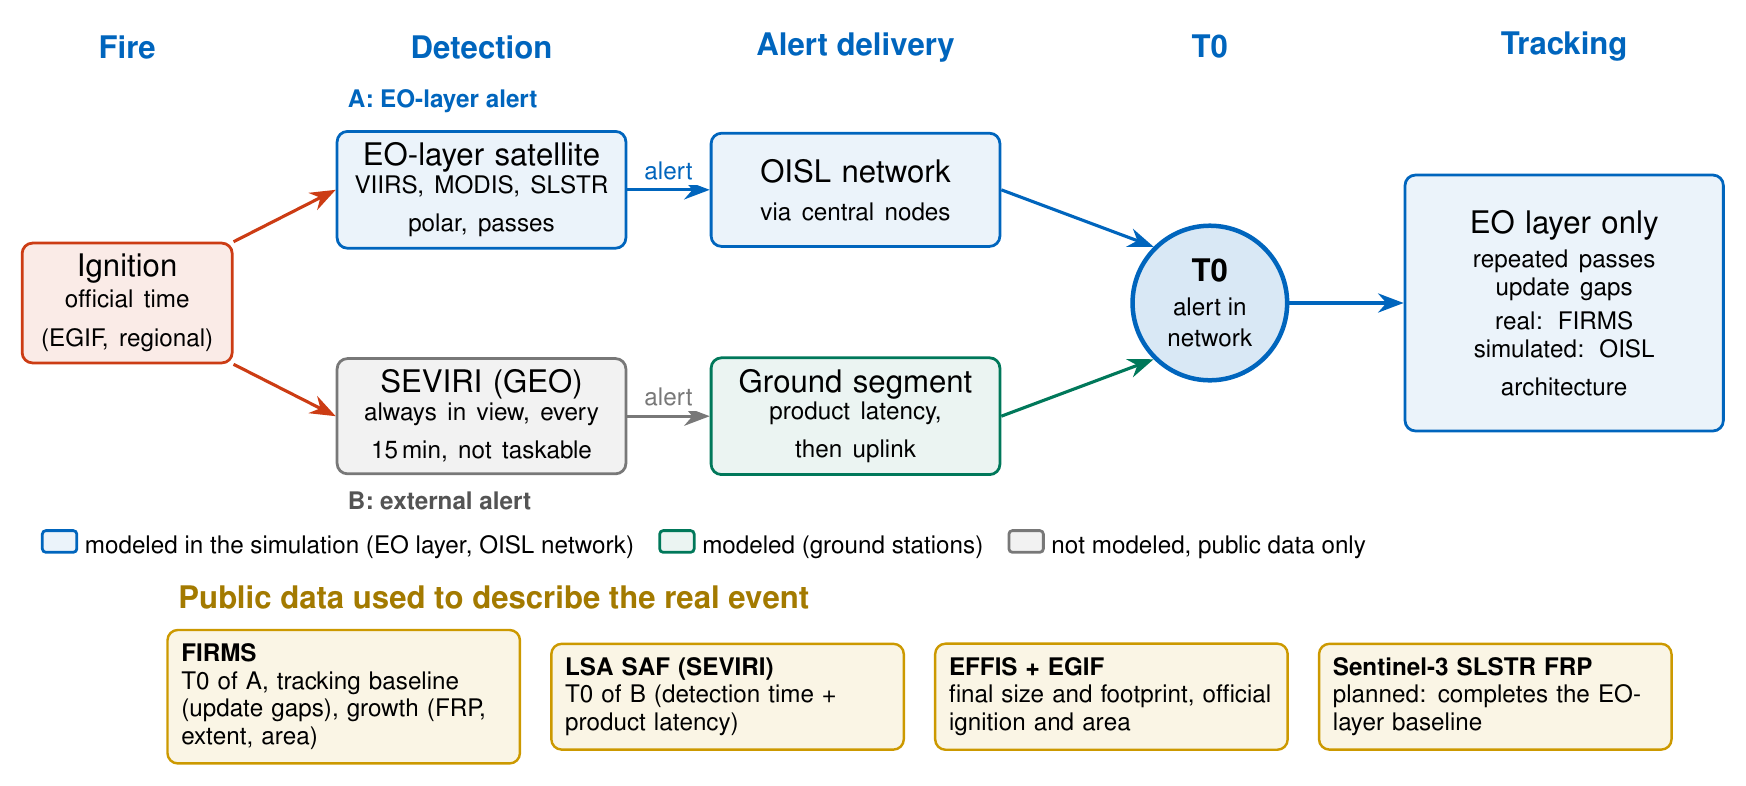
\includegraphics[width=\linewidth]{figures/alert_paths.png}
\caption{Alert paths and T0. Scenario A: an EO-layer satellite detects the fire and the alert travels through the OISL network. Scenario B: the geostationary SEVIRI detects the fire and the alert enters through the ground segment. In both scenarios tracking is done by the EO layer only. Blue and green elements are modeled in the simulation; grey elements are public data only. The bottom row shows which public dataset describes each part of the real event.}
\label{fig:alert_paths}
\end{figure}

SEVIRI is suited to the alert (always in view, every 15\,min) but not to tracking (coarse pixels, long blackouts, not taskable). In both scenarios the alert time is the detection time plus the product latency (FIRMS and LSA SAF processing and distribution), applied symmetrically. For a geostationary satellite the downlink itself is negligible, since it is in permanent ground contact. The values below are detection times; the official product latencies are still to be added.

\subsection{Methodology and rationale}
\label{subsec:baseline_method}

The goal is a \emph{public-record baseline}: for a real fire, when did existing satellites first observe it, and how often did they refresh that picture afterwards. These numbers are the benchmark for the OISL architecture. Pre-detection stays out of scope: T0 is the moment the alert enters the network.

The polar layer (Table~\ref{tab:sensing_layer}) is the only open, global, near-real-time active-fire record with per-pixel acquisition times, and it is the part of the problem that generalizes to events outside Europe. Its sun-synchronous passes cluster at fixed local times, which is the property the analysis exposes.

\textbf{Simplification.} Five polar platforms and one geostationary sensor are not the total coverage of a wildfire (Sentinel-2/3, commercial, airborne and ground sources also exist). This is a deliberate academic simplification; the problem stays the same with more sensors, because observing a fire is not delivering that information to the ground in time.

Each dataset has its own pipeline with a shared schema and event registry, so several events in the data window (8 to 16 Aug 2025) follow identical rules:
\begin{itemize}
  \item \textbf{Event selection}: a fire is a FIRMS cluster (1\,km grid, connected cells), seeded by the first detection near the official ignition point at or after the official ignition time. A box is only a crop: the Larouco box contained at least five fires and gave a first detection five days too early.
  \item \textbf{T0}: per alert path (Section~\ref{subsec:alert_paths}). Update gaps are measured from the scenario A T0.
  \item \textbf{Observation instants}: FIRMS, first event detection of each pass; SEVIRI, earliest acquisition time in each 15\,min slot with an event pixel.
  \item \textbf{Update gaps}: between consecutive instants from T0 to the last baseline instant; median, 90th percentile and maximum, also over a common horizon (47.7\,h after T0). Passes come in bursts, so the median alone hides the worst case.
  \item \textbf{Reproducibility}: all four pipelines reproduced the Larouco results exactly before processing Molezuelas.
\end{itemize}

\subsection{Results}
\label{subsec:baseline_results}

\begin{table}[!t]
\centering
\begin{tabular}{p{5.4cm} p{4.3cm} p{4.6cm}}
\hline
 & Larouco (Ourense) & Molezuelas / Castrocalb\'on (Zamora, Le\'on) \\
\hline
Official ignition (UTC) & 13 Aug 16:55 & 10 Aug 12:25 (approximate) \\
T0, scenario A (EO layer) & 13 Aug 21:45, Terra & 10 Aug 12:32, NOAA-20 \\
T0, scenario B (first of SEVIRI or EO layer) & 13 Aug 18:40, SEVIRI & 10 Aug 12:32, NOAA-20 \\
Ignition to T0, A / B & 4.83 / 1.75\,h & 0.12 / 0.12\,h \\
First SEVIRI detection & 18:40, 3.08\,h before A & 12:40, 0.13\,h after A \\
Observable window after T0 & 47.7\,h (end of FIRMS data) & 110.4\,h (last detection 15 Aug) \\
Baseline gaps, common horizon (median / p90 / max) & 0.85 / 6.17 / 8.60\,h & 0.60 / 6.13 / 7.63\,h \\
Baseline + SEVIRI, common horizon (max) & 8.60\,h & 4.48\,h \\
Longest SEVIRI blackout of the fire & 14.2\,h & 19.5\,h \\
Peak FRP in one pass & 26{,}563\,MW (NOAA-20) & 34{,}435\,MW (Aqua) \\
Forest area EGIF (Table~\ref{tab:events}) / EFFIS area & 37{,}765 / 37{,}179\,ha & 24{,}426 / 40{,}081\,ha \\
\hline
\end{tabular}
\caption{Public-record baseline for both events (times UTC, detection times without product latency). EGIF counts forest area only, EFFIS the full burnt area, so the two are not directly comparable.}
\label{tab:baseline_results}
\end{table}

\begin{figure}[!t]
\centering
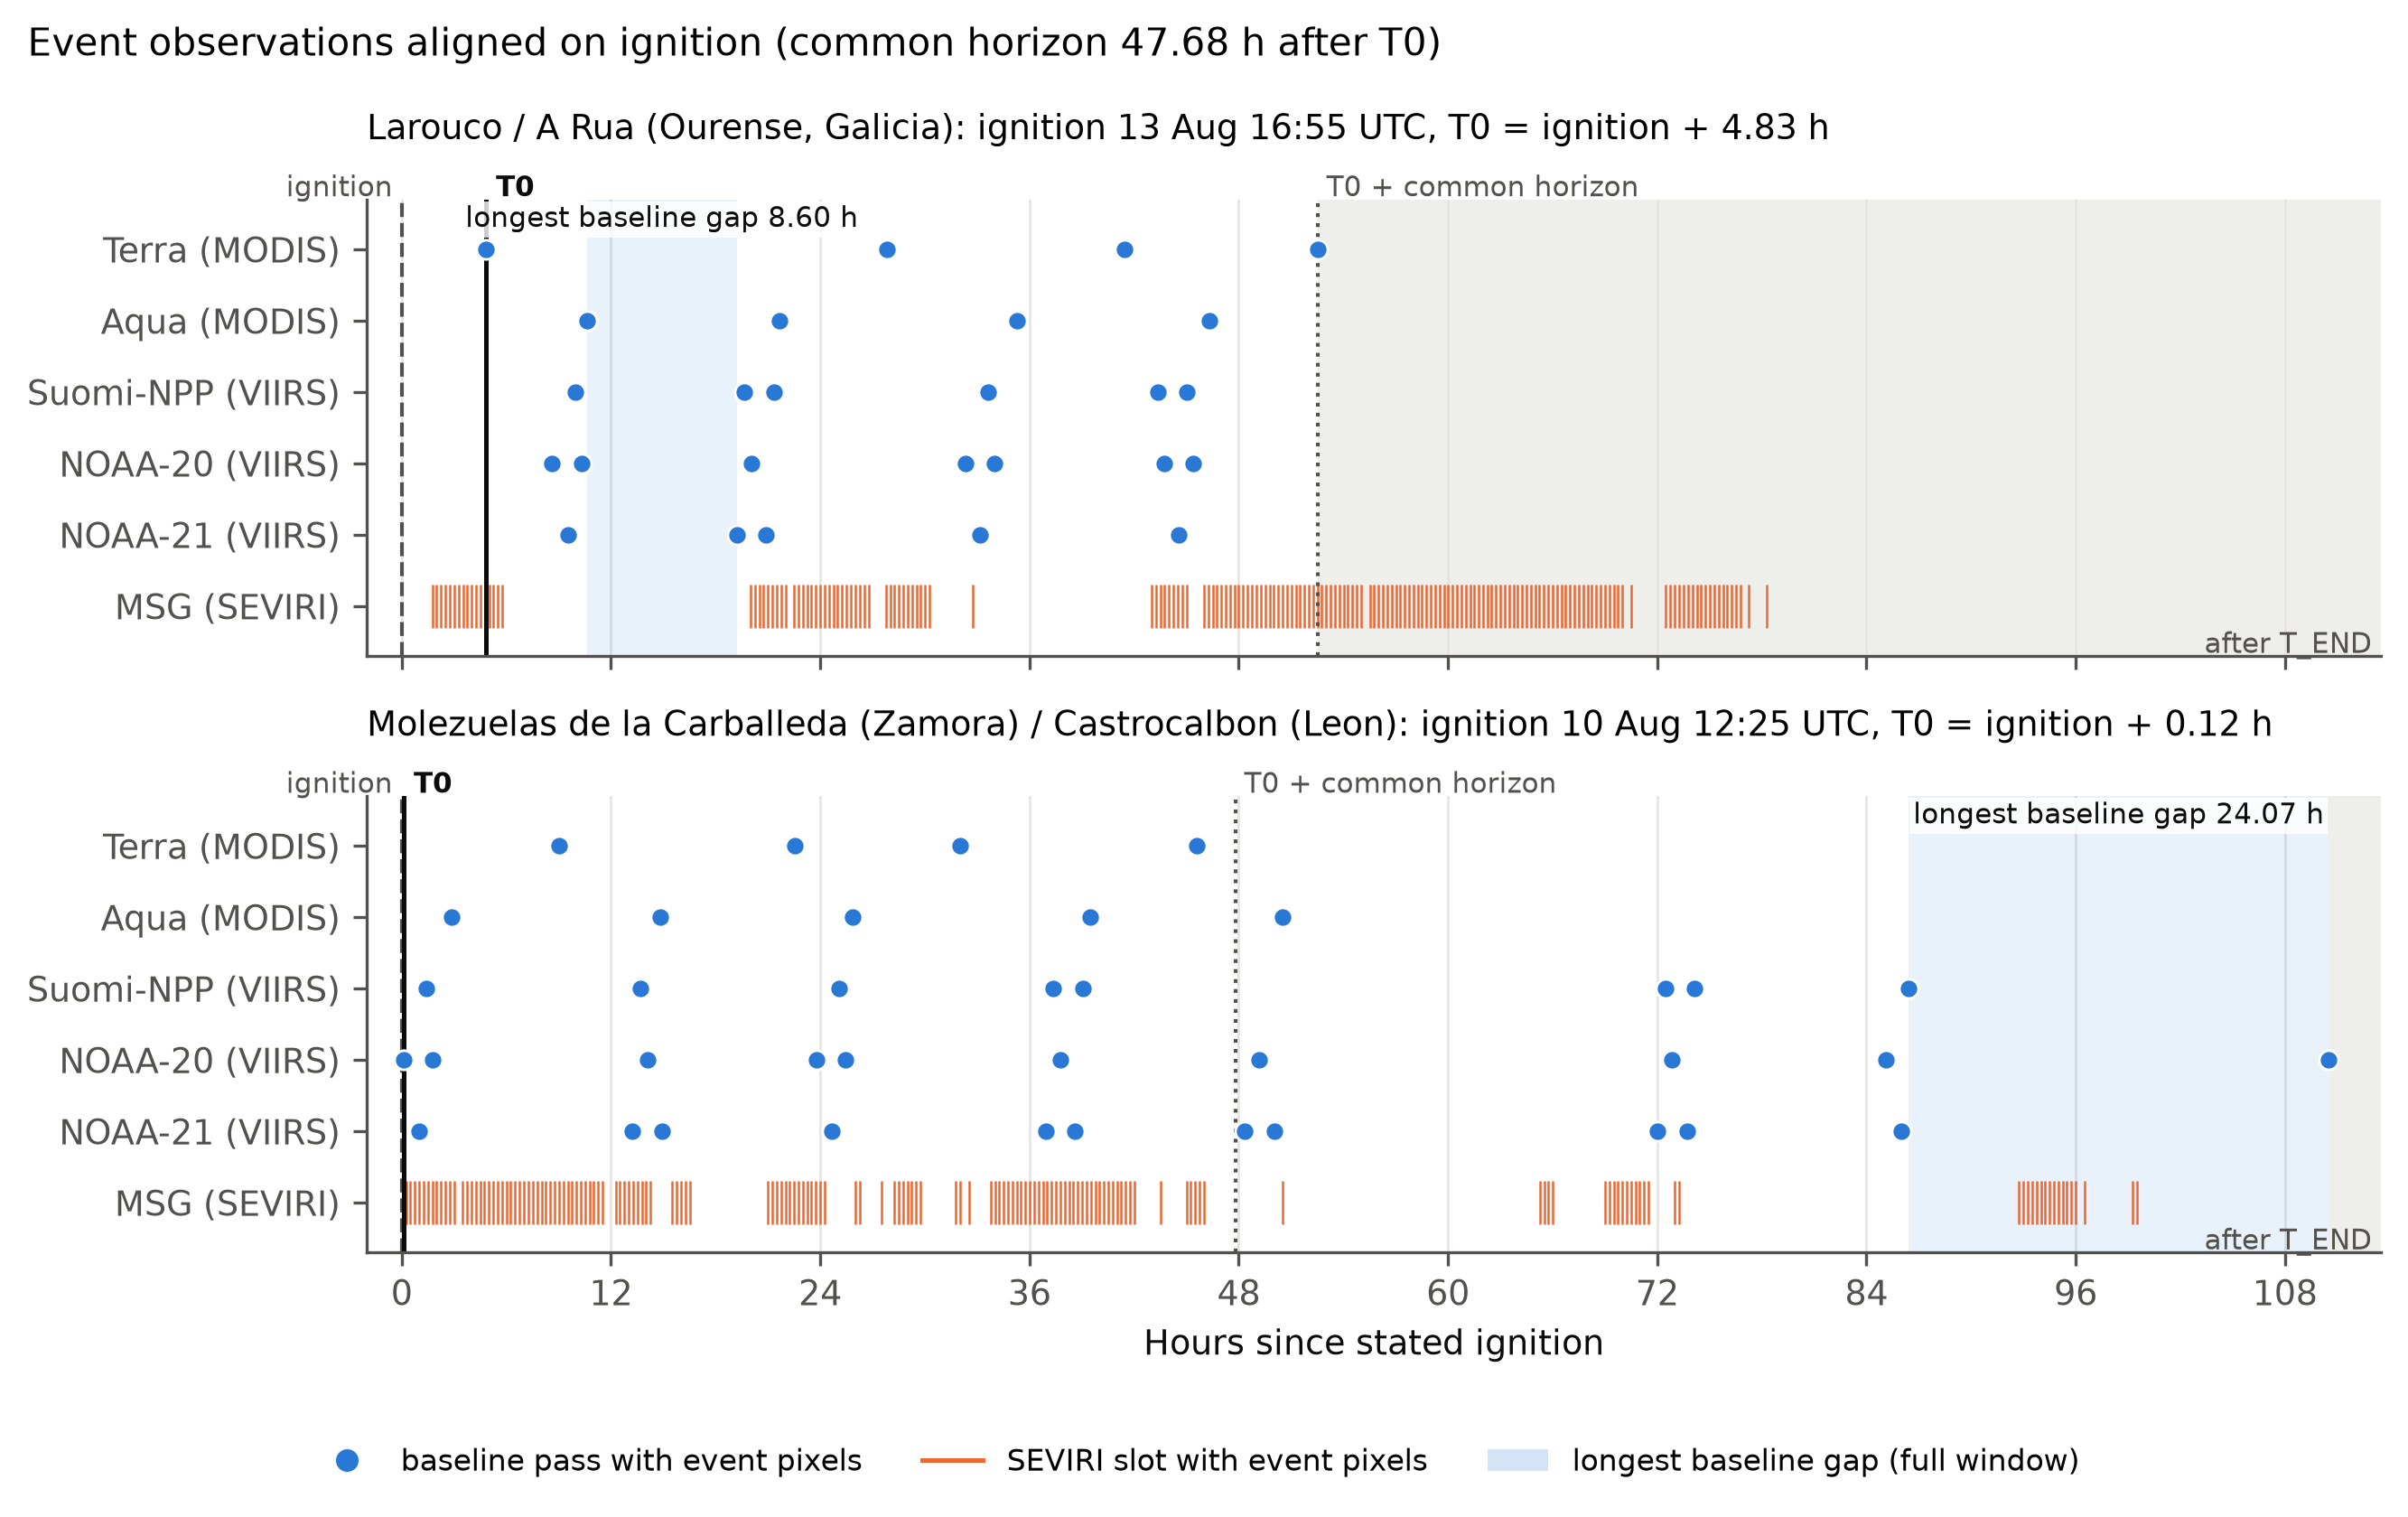
\includegraphics[width=0.72\linewidth]{figures/01_aligned_timelines.png}
\caption{Observation timelines of both events aligned at ignition: one row per platform plus SEVIRI, with T0 and the longest gap marked.}
\label{fig:aligned_timelines}
\end{figure}

\textbf{The worst gaps come from the orbit schedule, not from the fire.} Figure~\ref{fig:aligned_timelines} shows both timelines aligned at ignition. In both events, all eight baseline gaps of 6\,h or more inside the common horizon start between 03:21 and 04:11\,UTC or between 14:18 and 15:28\,UTC (Figure~\ref{fig:gaps_by_hour}). Inside a burst, passes arrive every 0.3 to 0.9\,h; between bursts, the wait is 6 to 8.6\,h. No single platform is a tracker: each updates the fire roughly twice a day.

\textbf{Alert latency depends on the ignition hour.} Molezuelas ignited minutes before an afternoon VIIRS pass (T0 after 0.12\,h); Larouco ignited just after the afternoon burst and waited 4.83\,h for the next Terra pass. In both cases the delay is entirely waiting for a pass: no pass missed the fire before T0. With an external alert (scenario B), Larouco's alert moves to 1.75\,h after ignition; Molezuelas does not change.

\textbf{Geostationary data alerts well but does not track.} SEVIRI saw Larouco 3.1\,h before the EO layer but then lost it for 14.2\,h, covering the whole 8.6\,h baseline hole. For Molezuelas it filled the holes during the first two days (combined maximum 4.48\,h), but lost the fire for up to 19.5\,h later. Most blackouts happen while SEVIRI still detects other fires nearby, so they reflect the fire being too small or obscured for 3 to 4\,km pixels, not a missing image.

\textbf{Growth and decay.} Molezuelas spread north-east into Le\'on (27\,km, 34{,}435\,MW on 12 Aug; Figure~\ref{fig:molezuelas_map}), then fell below FIRMS detection while officially active until about 22 Aug. Its full-window maximum gap (24.1\,h) reflects decay, not revisit.

\textbf{EFFIS is a reference, not a validation.} 96\% of Spanish EFFIS start dates coincide with a FIRMS pass (for Molezuelas it is the T0 detection itself). Area figures differ by definition (forest area, full burnt area, regional or multi-province totals), so EFFIS areas are quoted as a reference only.



\begin{figure}[!t]
\centering
\begin{minipage}[t]{0.49\linewidth}
\centering
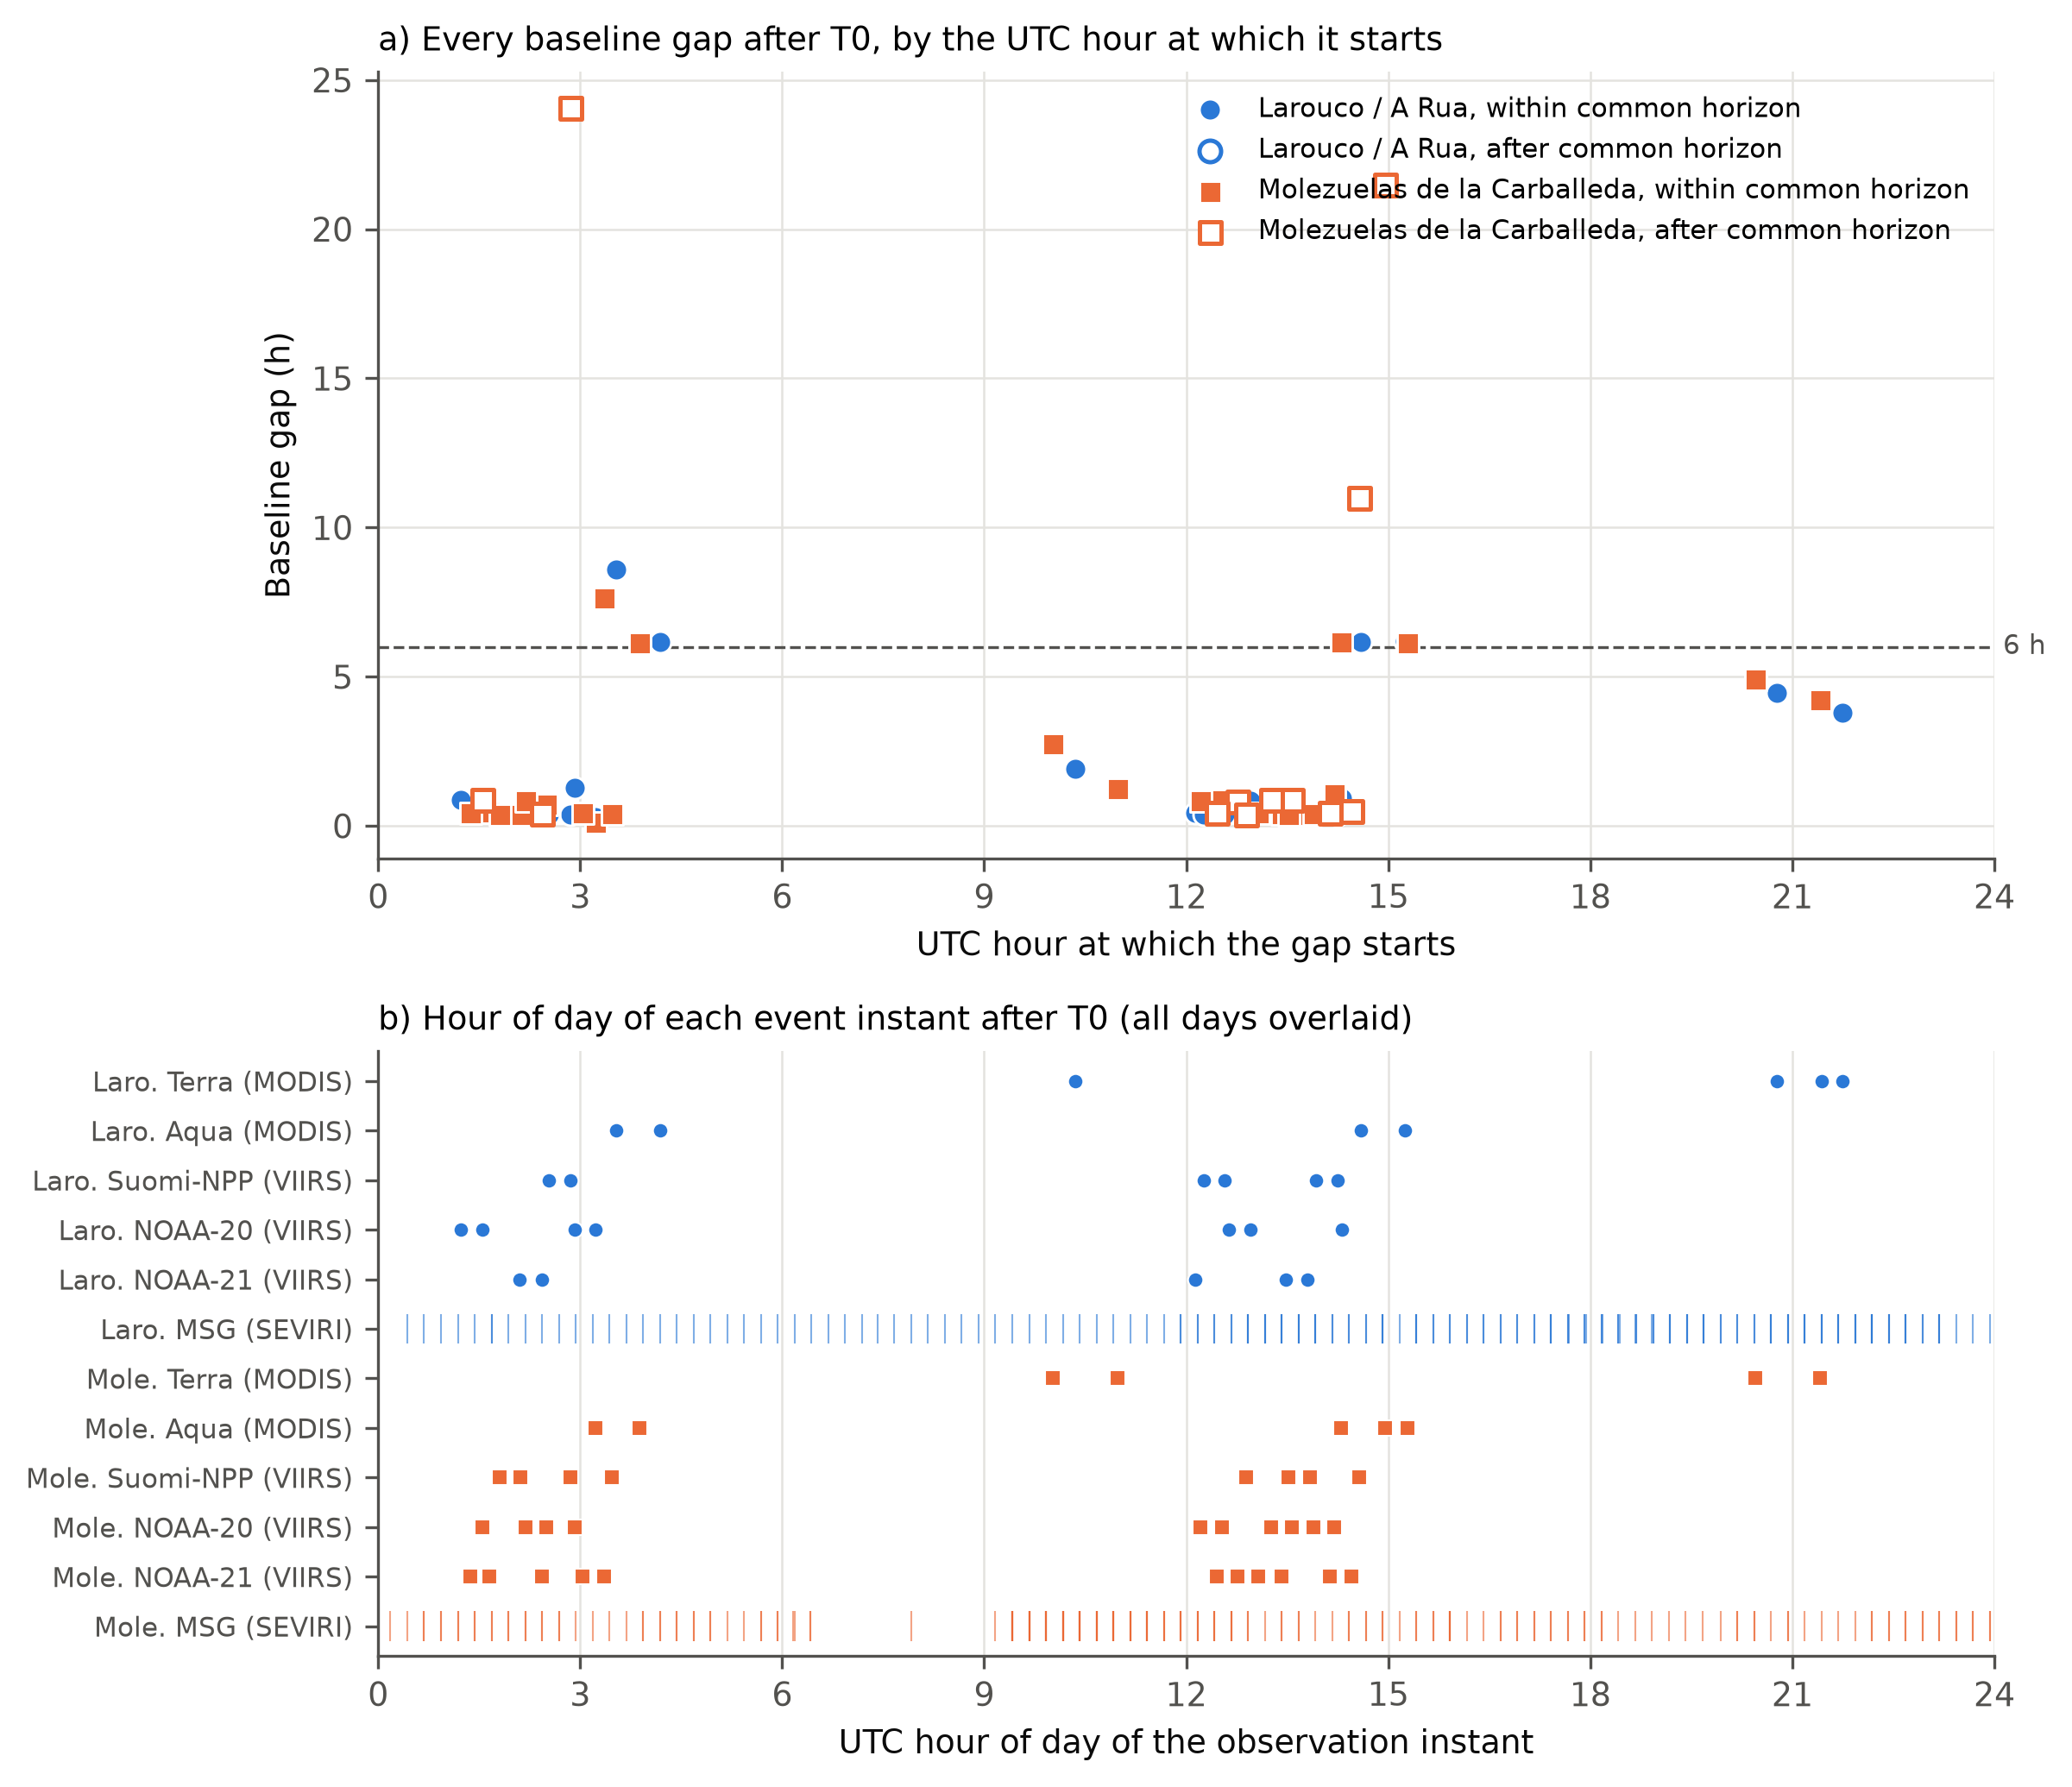
\includegraphics[width=\linewidth]{figures/02_gaps_by_hour.png}
\caption{Baseline update gaps by UTC start hour, both events. Long gaps cluster at fixed hours set by the polar orbit schedule.}
\label{fig:gaps_by_hour}
\end{minipage}\hfill
\begin{minipage}[t]{0.49\linewidth}
\centering
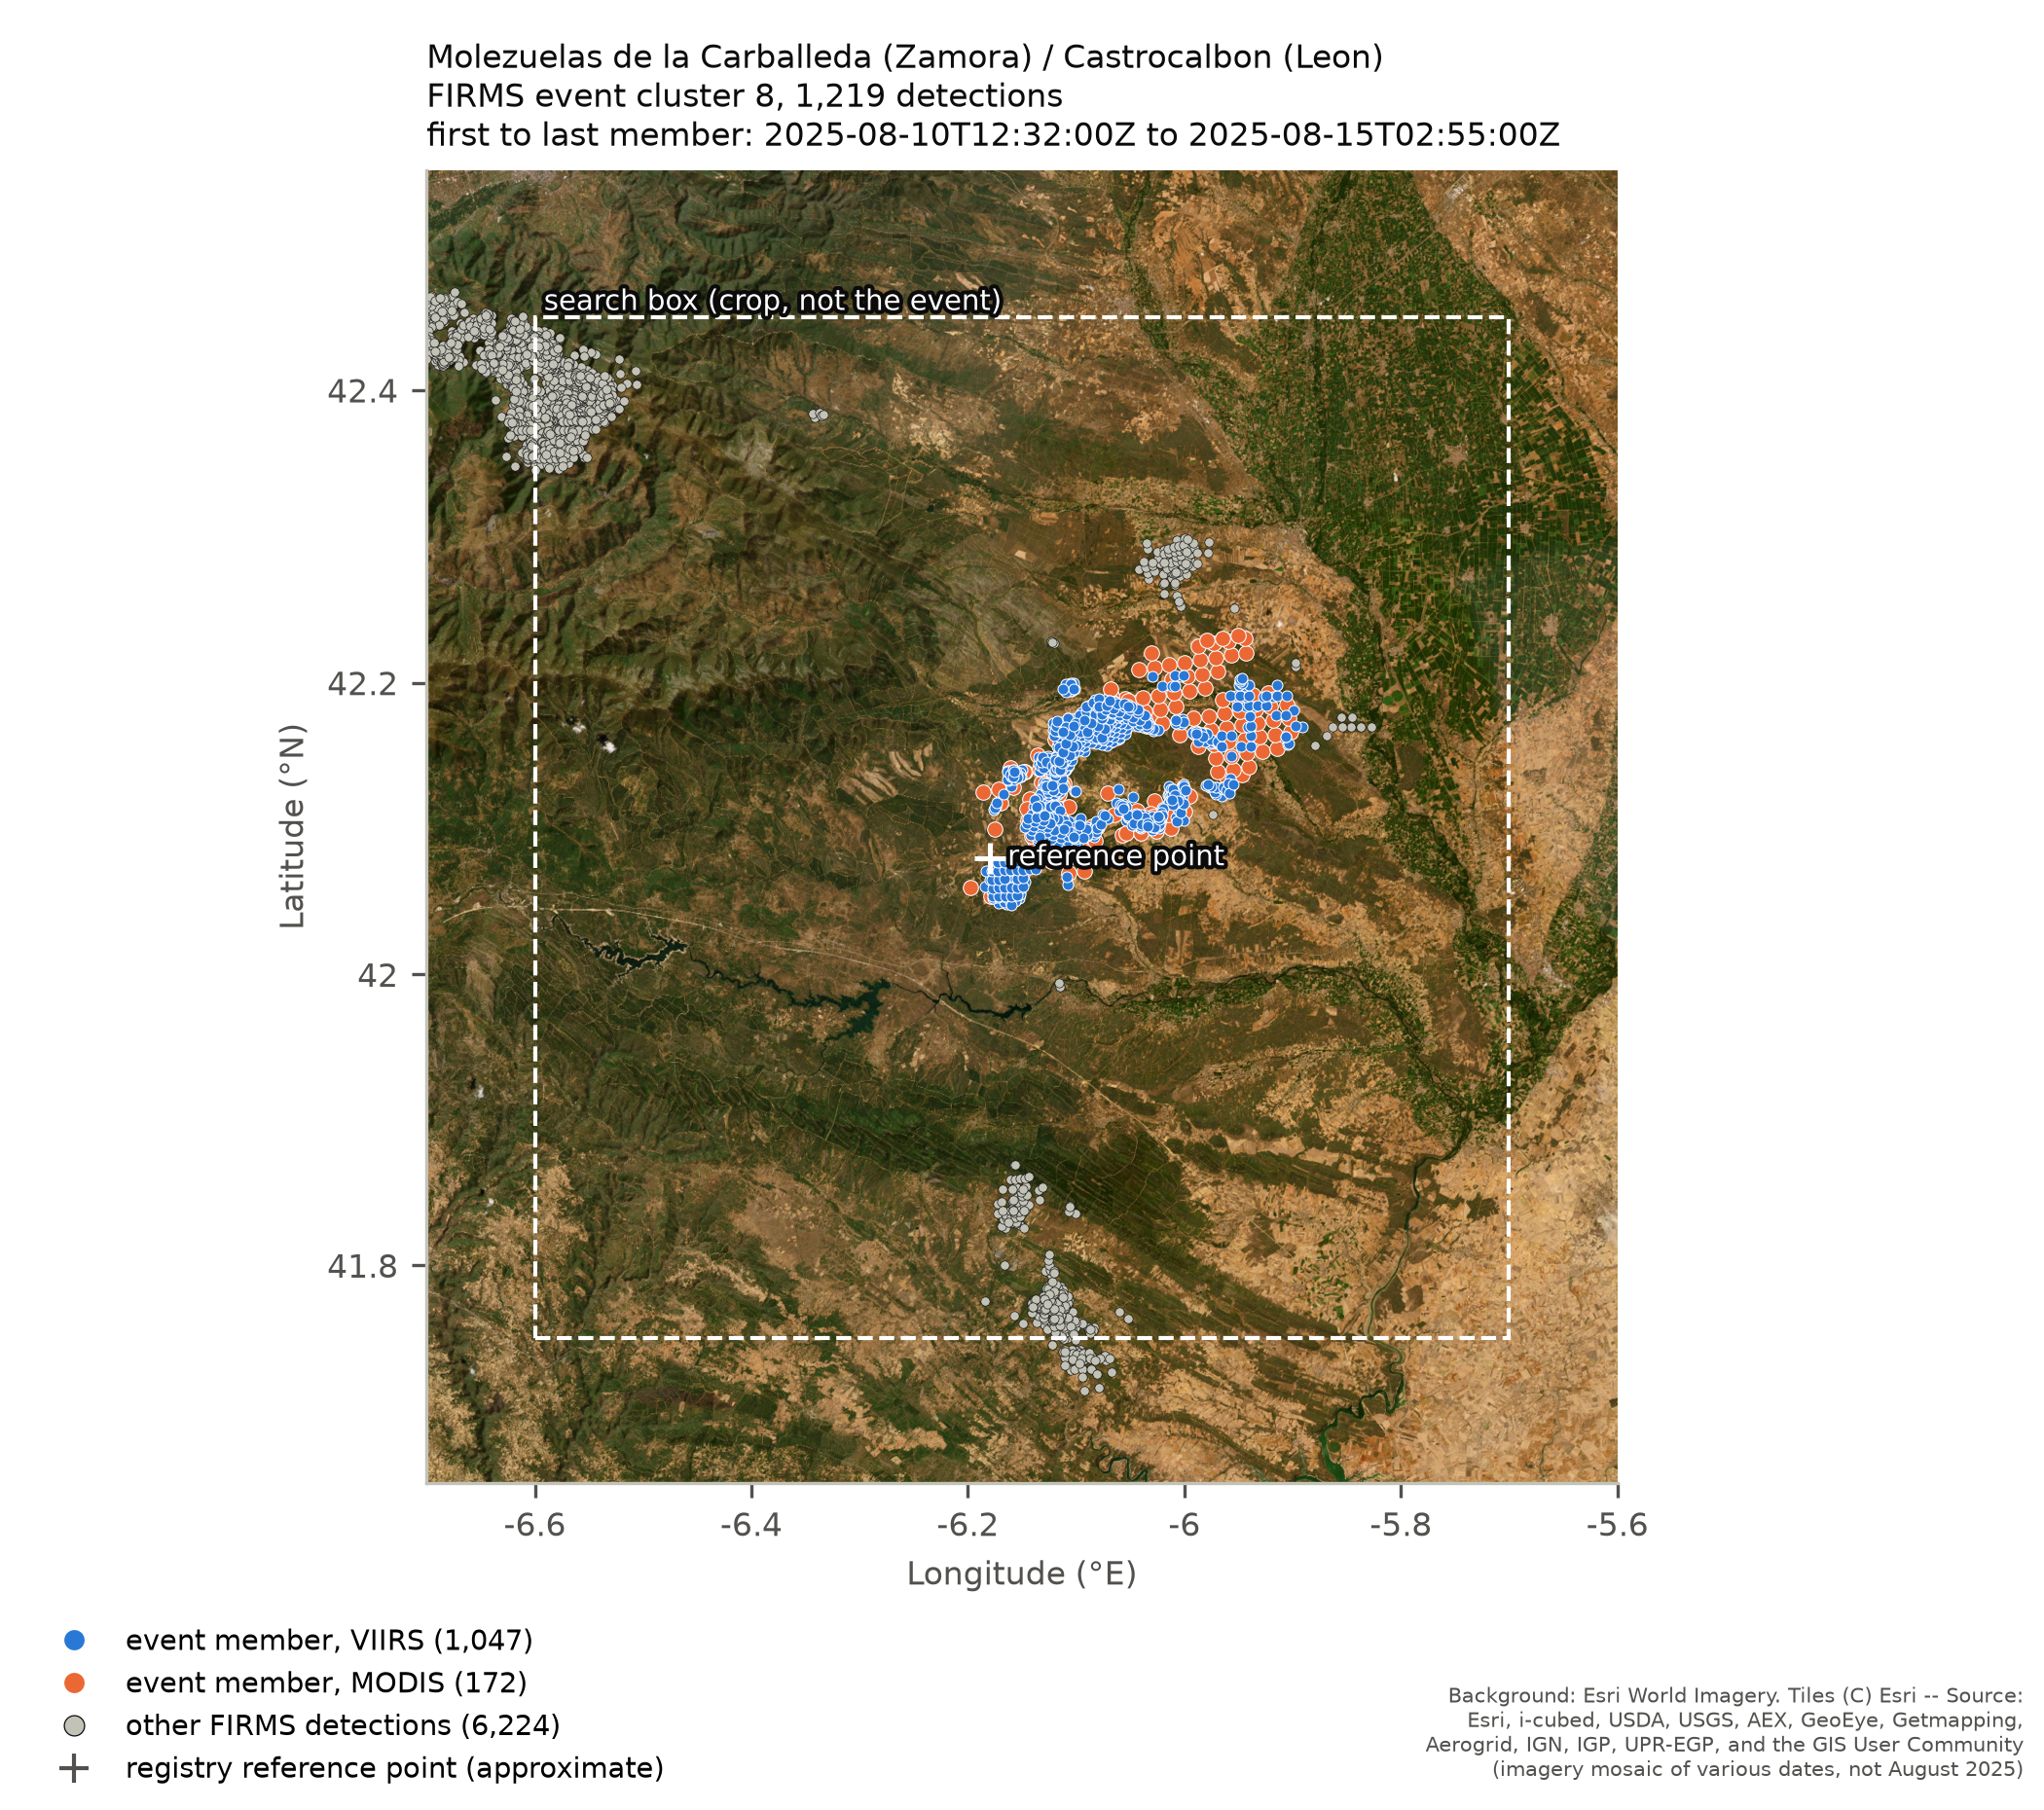
\includegraphics[width=\linewidth]{figures/01_map_event.png}
\caption{Molezuelas: FIRMS event detections (cluster) and other detections in the search box. Background is an older mosaic, not August 2025.}
\label{fig:molezuelas_map}
\end{minipage}
\end{figure}

\subsection{How the results answer the research questions}
\label{subsec:baseline_rq}

\begin{itemize}
  \item \textbf{First observation timing}: in scenario A set by the ignition hour against the pass schedule (0.12 to 4.83\,h), not by the fire; an external geostationary alert (scenario B) can shorten it, but tracking still depends on the EO layer.
  \item \textbf{Coverage versus decentralization}: the target is the recurring 6 to 8.6\,h holes (about 03 to 12 and 15 to 21\,UTC); observing and reporting inside them beats the whole public record on the worst case.
  \item \textbf{Latency components}: all gaps are \emph{observation} times; processing and downlink come on top, so the delivered record is slower. Even with perfect observation, an EO satellite cannot downlink without a ground station in view: the gap OISL relay and central-node placement address.
  \item \textbf{Task reprioritization}: FRP and extent per pass show when a fire changes state (Molezuelas peak on 12 Aug), i.e.\ the information that should trigger re-tasking.
\end{itemize}

\subsection{Open questions and next steps}
\label{subsec:baseline_next}

\begin{itemize}
  \item \actionitem{Cross-check with the EO layer of the NeuralAgent simulator (Section~\ref{sec:eo}): simulated access windows of the five baseline platforms must contain every observed pass. The simulation adds the passes without detection, and the Sentinel-3 passes, that the public record cannot show.}
  \item \actionitem{Run the OISL architecture against the benchmark (Table~\ref{tab:baseline_results}) over the common horizon, including the downlink latency.}
  \item \vincenzoq{Which alert path should the thesis study: the EO-layer alert (scenario A, Month 1 assumption), the external alert through the ground segment (scenario B), or both as two scenarios? For Larouco the alert time differs by 3.1\,h; gap statistics are not affected.}
  \item \vincenzoq{Will task prioritization in the simulation use fire size? This decides how much growth modeling is needed beyond the FIRMS-based cumulative area.}
  \item \actionitem{Add the official product latencies of FIRMS and LSA SAF to the detection times of both alert paths.}
  \item \actionitem{Download Sentinel-3 SLSTR FRP for 8 to 16 Aug 2025 and check for daytime detections, since the near-real-time product was documented as mainly night-time. If usable, add it to the baseline as a fifth pipeline.}
  \item \actionitem{Re-request EFFIS burnt areas with perimeters (shapefile) for the final footprint of both events.}
  \item \actionitem{Compute the cumulative FIRMS VIIRS detection area per day as growth proxy.}
  \item \openquestion{Verify the Molezuelas ignition time (approximate, from press reports of Junta de Castilla y Le\'on).}
  \item \openquestion{Extend FIRMS and LSA SAF beyond 15 Aug to track all of Larouco?}
\end{itemize}

% =========================================================
\section{Next Steps}
% =========================================================

\begin{itemize}[leftmargin=1.2cm]
    \item \actionitem{Verify the complexity model with Vincenzo and do an initial code implementation (Section~\ref{sec:complexity}).}
    \item \actionitem{Pull observation and communication time windows from OrbiNet for the candidate scenarios, now including FOV and the five ground stations.}
    \item \actionitem{Cross-check the simulated EO layer against the public-record baseline for both events (Section~\ref{subsec:baseline_next}).}
    \item \actionitem{Support both alert paths in the simulation: alert injected by an EO-layer satellite (A) or through a ground station (B).}
    \item \actionitem{Complete the baseline with Sentinel-3 SLSTR FRP and the EFFIS perimeters.}
    \item \actionitem{Resolve the open link-type points, in particular the sensing-to-coordination link (Section~\ref{subsec:bandopen}).}
\end{itemize}

Action items coming from meeting with Vincenzo on the 20th of October:
\begin{itemize}
    \item \actionitem{Identify what are the limitations of existing observations.}
    \item \actionitem{Including revisit time, estimated latency, sensor wavelength, resolution.}
    \item \actionitem{Can we check from the declared wildfire starting time, how much time passes before the first satellite can do the observation?}
    \item \actionitem{Classify and simulate the performances achievable from existing satellites in terms of revisit time and latency with the guessed suggestions.}
    \item \actionitem{Ground station link can be maybe implemented as postprocessing. So initially we consider all the comm link valid and then we exclude some of them in the postprocessing.}
    \item \actionitem{Propose structural complexity metrics alpha for different nodes and GS (Section~\ref{sec:complexity}).}
    \item \actionitem{Propose also values or an equation for defining the complexity of links (beta) (Section~\ref{sec:complexity})}
    \item \actionitem{[The link band can be fixed based on existing missions, similar mission or NeuralAgent architecture suggestion] }
    \item \vincenzoq{What would be the difference between my coordination layer and the CN? What it is really the task of the CNs? How would they communicate with each other? Can the sensing layer talk with the coordination layer? Can the coordination layer talk to the GS?}
    \item \actionitem{Research pixel size accuracy for each sensor in EO}
    \item \actionitem{Research companies in the wilfire business such as \textbf{Auroratech} and \textbf{PlanetLab} and try to get the tle of their satellites to see if we implement them too as a third layer of private business providers}
\end{itemize}

Decisions agreed on:
\begin{itemize}
    \item EO layer will just use RF, not Optical ISL.
\end{itemize}
\printbibliography

\end{document}